\documentclass[10pt,twocolumn,letterpaper]{article}

\usepackage{cvpr}
\usepackage{times}
\usepackage{epsfig}
\usepackage{graphicx}
\usepackage{amsmath}
\usepackage{amssymb}

% Include other packages here, before hyperref.

% If you comment hyperref and then uncomment it, you should delete
% egpaper.aux before re-running latex.  (Or just hit 'q' on the first latex
% run, let it finish, and you should be clear).
\usepackage[breaklinks=true,bookmarks=false]{hyperref}

\cvprfinalcopy % *** Uncomment this line for the final submission

\def\cvprPaperID{****} % *** Enter the CVPR Paper ID here
\def\httilde{\mbox{\tt\raisebox{-.5ex}{\symbol{126}}}}

% Pages are numbered in submission mode, and unnumbered in camera-ready
%\ifcvprfinal\pagestyle{empty}\fi
\setcounter{page}{1}
\begin{document}

%%%%%%%%% TITLE
\title{Evaluation of SD Filter for Multi-Spectral Image De-Noising}

\author{Mert Can Ergun\\
Hacettepe University\\
Department of Computer Engineering\\
{\tt\small mcergun@windowslive.com}
% For a paper whose authors are all at the same institution,
% omit the following lines up until the closing ``}''.
% Additional authors and addresses can be added with ``\and'',
% just like the second author.
% To save space, use either the email address or home page, not both
\and
Gokhan Yaliniz\\
Hacettepe University\\
Department of Computer Engineering\\
{\tt\small gokhanyaliniz@gmail.com}
}

\maketitle
%\thispagestyle{empty}

%%%%%%%%% ABSTRACT
\begin{abstract}
   Traditional de-noising algorithms using static and dynamic guidance images are already used. The SD Filter leverages both static and dynamic guidance together for many applications. For this project de-noising application is studied. The method uses high detail NIR image as a static guidance for de-noising an visible spectrum RGB image.
   
   To evaluate this method's performance some image metric methods are also studied in this paper.
\end{abstract}

%%%%%%%%% BODY TEXT
\section{Introduction}

Many tasks in image processing requires regularization in order to get good results. Guidance is used to transfer strong structures from one image to another. 

Traditional methods use static or dynamic guidance images. Static guidance regularization modulates input image with similarities between two images. It can easily reflect internal properties of the input image.
Dynamic guidance regularization on the other hand modulates input image with similarities between neighboring pixels. It can preserve local features better than static guidance regularization.

Robust Image Filtering using Joint Static and Dynamic Guidance\cite{ham2015} paper uses both static and dynamic guidance images together to keep local features and static image structures intact.

Infrared sensors are still developing and thus there are some intrinsic problems with Infrared Imaging(IR). These problems will be dealt with during the project.

TRICLOBS(TRI-band Color Low-light OBServation) Dataset\cite{triclobs} is used for de-noising with multiple spectrum images of the same scene. The dataset includes different civilian or military scenarios executed against a special kind of hardware that records visible, NIR and LWIR spectrum. This database will be used in evaluation part of the method\cite{ham2015}.

%-------------------------------------------------------------------------
\section{Related Work}
Lorem ipsum dolor sit amet, consectetur adipiscing elit. Maecenas nec porta orci, eu porta velit. Morbi pulvinar, tortor vitae venenatis laoreet, elit ligula vehicula augue, non luctus ipsum eros eu massa. Fusce non sem varius sem sodales dapibus. Mauris urna mi, ullamcorper eget nisl vel, imperdiet lacinia dolor. Nulla facilisi. Maecenas volutpat augue suscipit ultrices hendrerit. Vestibulum suscipit diam condimentum porttitor consectetur. Etiam sit amet libero sed erat sollicitudin lobortis vitae non quam. Quisque porta sodales enim, sed malesuada mauris viverra vestibulum. Cras tempor vehicula libero at aliquet.

Aliquam erat volutpat. Vestibulum pellentesque eros odio, in porta enim finibus quis. Curabitur sagittis urna et neque consectetur rutrum. Aenean pharetra efficitur accumsan. Aliquam erat volutpat. Vestibulum at dolor laoreet felis molestie sodales. Morbi dapibus quis elit sit amet aliquet. Duis vitae lorem at risus bibendum vehicula. Vestibulum neque urna, accumsan sagittis massa nec, vestibulum condimentum nisl. Pellentesque id purus vel nibh consectetur cursus. Aenean ornare erat urna, sit amet pharetra urna feugiat non. Quisque mattis, odio sed eleifend lacinia, sem leo venenatis leo, nec congue nulla nisi vitae ante. Duis aliquam sollicitudin aliquam.

Nam nisl nunc, efficitur a dolor et, semper convallis erat. Proin lobortis posuere turpis non pharetra. In hac habitasse platea dictumst. Maecenas finibus, nibh vitae egestas egestas, libero neque semper enim, ac venenatis metus quam non dui. Ut blandit ultrices ultrices. Mauris est neque, malesuada sed ullamcorper quis, blandit mollis mi. Nunc id lobortis sapien. Maecenas a malesuada ipsum. Orci varius natoque penatibus et magnis dis parturient montes, nascetur ridiculus mus. Suspendisse efficitur justo sit amet enim euismod accumsan. Interdum et malesuada fames ac ante ipsum primis in faucibus. Mauris non ligula efficitur urna egestas euismod. Aenean semper quis lectus nec fringilla. Duis luctus sem gravida commodo malesuada. Duis consequat sollicitudin imperdiet.

\section{Methodology}
The project can be divided into two main parts. The methodology for each part will be discussed in following sections.

\subsection{Sigma Estimation}
IR imaging sensors are more complicated than visible light RGB sensors. One of the problems of IR sensors is higher amounts of noise.
For most image processing applications, especially for image de-noising, there needs to be a way to measure image quality and enhancements between pre-algorithm and post-algorithm steps.

A widely used image quality metric is peak signal to noise ratio(PSNR). PSNR, is an engineering term for the ratio between the maximum possible power of a signal and the power of corrupting noise that affects the fidelity of its representation\cite{psnr-wiki}. For SNR measurements to work correctly, original image needs to be virtually noise-free.

Since original images are noisy in our case we will use two different methods to estimate noise levels from the original image. Then noise levels will be used as an image quality metric. Both methods were originally meant for additive white gaussian noise, this may or may not be the case for our dataset. Thus these methods need to be evaluated as well.
\subsubsection{Online Variance Calculation on Consecutive Frames}
\subsubsection{Noise Level Estimation Using Weak Textured Patches of a Single Noisy Image}
\begin{figure}
	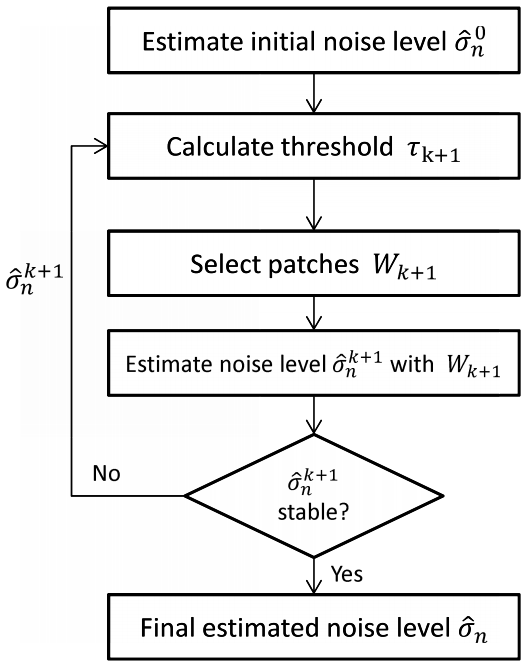
\includegraphics[width=0.9\columnwidth]{single_image_noise_estimation.png}
	\caption{Algorithm for \cite{noise-weak-texture}.}
	\label{fig:alg-weak-texture}
\end{figure}
Noise Level Estimation Using Weak Textured Patches of a Single Noisy Image\cite{noise-weak-texture} uses low rank weak textured patches without high frequency components. Noise level is then estimated from selected patches using principal component analysis(PCA). Figure \ref{fig:alg-weak-texture} shows the overall algorithm for this method.

\subsection{Filtering Framework}
Lorem ipsum dolor sit amet, consectetur adipiscing elit. Maecenas nec porta orci, eu porta velit. Morbi pulvinar, tortor vitae venenatis laoreet, elit ligula vehicula augue, non luctus ipsum eros eu massa. Fusce non sem varius sem sodales dapibus. Mauris urna mi, ullamcorper eget nisl vel, imperdiet lacinia dolor. Nulla facilisi. Maecenas volutpat augue suscipit ultrices hendrerit. Vestibulum suscipit diam condimentum porttitor consectetur. Etiam sit amet libero sed erat sollicitudin lobortis vitae non quam. Quisque porta sodales enim, sed malesuada mauris viverra vestibulum. Cras tempor vehicula libero at aliquet.

Aliquam erat volutpat. Vestibulum pellentesque eros odio, in porta enim finibus quis. Curabitur sagittis urna et neque consectetur rutrum. Aenean pharetra efficitur accumsan. Aliquam erat volutpat. Vestibulum at dolor laoreet felis molestie sodales. Morbi dapibus quis elit sit amet aliquet. Duis vitae lorem at risus bibendum vehicula. Vestibulum neque urna, accumsan sagittis massa nec, vestibulum condimentum nisl. Pellentesque id purus vel nibh consectetur cursus. Aenean ornare erat urna, sit amet pharetra urna feugiat non. Quisque mattis, odio sed eleifend lacinia, sem leo venenatis leo, nec congue nulla nisi vitae ante. Duis aliquam sollicitudin aliquam.

Nam nisl nunc, efficitur a dolor et, semper convallis erat. Proin lobortis posuere turpis non pharetra. In hac habitasse platea dictumst. Maecenas finibus, nibh vitae egestas egestas, libero neque semper enim, ac venenatis metus quam non dui. Ut blandit ultrices ultrices. Mauris est neque, malesuada sed ullamcorper quis, blandit mollis mi. Nunc id lobortis sapien. Maecenas a malesuada ipsum. Orci varius natoque penatibus et magnis dis parturient montes, nascetur ridiculus mus. Suspendisse efficitur justo sit amet enim euismod accumsan. Interdum et malesuada fames ac ante ipsum primis in faucibus. Mauris non ligula efficitur urna egestas euismod. Aenean semper quis lectus nec fringilla. Duis luctus sem gravida commodo malesuada. Duis consequat sollicitudin imperdiet.

\section{Experiments}


{\small
\bibliographystyle{ieee}
\bibliography{egbib}
}

\end{document}
